\section{Parameter-Based Non-Stationary Policy Optimisation for Delays}


\subsection{Lifelong Parameter-Based Policy Optimisation}
\label{sec:lifelong_param_po}

In this section, we build on the parameter-based \gls{po} and consider a hyper-policy in $\mathcal{V}_{\mathcal{P}} = \{\nu_{\vectorialform{\rho}} : \vectorialform{\rho} \in \mathcal{P} \subseteq \realnumbers^{n_\rho}\}$ and a policy in $\Pi_{\Theta} = \{\pi_{\vectorialform{\theta}} : \vectorialform{\theta} \in \Theta \subseteq \realnumbers^{n_\theta}\}$.
In order to optimise for the $\beta$-step ahead expected return of \Cref{eq:beta_steps_ahead_return} the policy must be non-stationary.
This can be done in two ways using the parameter-based \gls{po} framework.  
In the first, the state $s$ is augmented with the current time $t$ yielding policies $a_t\sim\pi_{\boldsymbol\theta}(\cdot\vert(s,t))$.
This formulation clearly shows the dependence of the action on time. 
In the second, the dependence on time is moved to the hyper-policy level, and therefore the parameters of the policy depend on time $\boldsymbol\theta_t \sim \nu_{\boldsymbol\rho}(\cdot\vert t)$.
This arguably provides a better understanding on how the agent adapts to the non-stationarity.
A graphical representation of the two frameworks is given in \Cref{fig:graph_models}.
We call this setting the \emph{lifelong parameter-based PO}.


\begin{figure}[t]
    \centering
    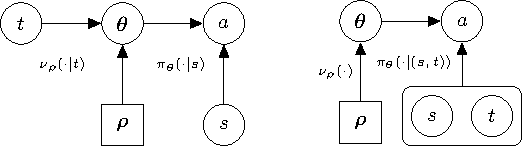
\includegraphics[labellifelong=graphparamactionbasedns]{img/thesis_plots_chapter_lifelong.pdf}
    \caption{Graphical models representing the two frameworks of parameter-based \gls{po} applied to a non-stationarity of the environment. Left, non-stationarity is handled at the policy parameter level; right, non-stationarity is handled at the action level.}
    \label{fig:graph_models}
\end{figure}

The $\beta$-step ahead expected return can be reformulated for parameter-based \gls{po} as:
\begin{align}\label{eq:opt}
	\boldsymbol\rho^\star_{T,\beta} \in \argmax_{\boldsymbol\rho \in \mathcal{P}} \expectedreturn[T,\beta][](\boldsymbol\rho) = \sum_{t=T+1}^{T+\beta} \widehat{\gamma}^t \expectedvalue_t^{\boldsymbol\rho}[r_t],
\end{align} 
where $\mathbb{E}_t^{\boldsymbol\rho}\coloneq \expectedvalue_{\boldsymbol\theta \sim \nu_{\boldsymbol\rho}(\cdot\vert t)}[\mathbb{E}_t^{\pi_{\boldsymbol\theta}}[\cdot]]$.


\subsection{Lifelong Parameter-Based PO via Multiple Importance Sampling}
\label{subsec:mis_lifelong}

We now propose an approach to optimise for the $\beta$-step ahead expected return. 
In \Cref{subsec:beta_step_estim}, we derive an estimator for this quantity.
In \Cref{subsec:bias_analysis}, we analyse the bias of the estimator and in \Cref{subsec:variance_analysis} its variance.
Finally, in \Cref{subsec:surrogate_objective}, we propose a surrogate objective that accounts for the uncertainty of the estimation to optimise a lower bound of $\expectedreturn[T,\beta][](\boldsymbol\rho)$.

\subsubsection{$\beta$-Step Ahead Expected Return Estimator}
\label{subsec:beta_step_estim}

Obviously, the challenge here is to estimate a quantity which depends on future unknown dynamics having access only to past samples when dynamics were potentially different. 
However, assuming smoothness in the non-stationarity--which we do assume here--makes it reasonable to use past dynamics in order to predict future ones. 
More formally, let $\mathcal{H}_{T,\alpha} = (\boldsymbol\theta_t,r_t)_{t \in [\![T-\alpha+1,T]\!]}$ be the last $\alpha$ samples of the lifelong interaction with the environment.
Using these samples and \gls{mis}, one can build a (biased) estimator of the $s$-step ahead expected reward $\mathbb{E}_s^{\boldsymbol\rho}[r_s]$ for $s \in [\![T+1,T+\beta]\!]$:
\begin{align*}
    \widehat{r}_{s} = \sum_{t=T-\alpha+1}^{T} \omega^{T-t} \frac{\nu_{\boldsymbol\rho}(\boldsymbol\theta_t\vert s)}{ \sum_{k=T-\alpha+1}^T \omega^{T-k} \nu_{\boldsymbol\rho}(\boldsymbol\theta_t\vert k)} r_{t},
\end{align*}
where $\omega \in [0,1]$ is an exponential discounting parameter.
Note that here, the importance sampling weights $\textstyle\frac{\nu_{\boldsymbol\rho}(\boldsymbol\theta_t\vert s)}{ \sum_{k=T-\alpha+1}^T \omega^{T-k} \nu_{\boldsymbol\rho}(\boldsymbol\theta_k\vert k)}$ account for the discrepancy between target hyper-policies in the future $\nu_{\boldsymbol\rho}(\cdot\vert s)$ and the behavioural hyper-policies from the past $\nu_{\boldsymbol\rho}(\cdot\vert k)$. 
Due to the $\omega$ discounting, the \gls{mis} estimator does not exactly use the coefficient suggested by BH (see~\Cref{subsec:importance_sampling}). 
Instead, it embodies our knowledge that the environment changes smoothly by giving more weight to recent samples. BH instead would weigh each past sample equally. 
The exponential discounting of samples as they get older is not novel in non-stationary environments \cite{jagerman2019people}.

One can now leverage the estimator $\widehat{r}_{s}$ to estimate the $\beta$-step ahead expected return,
\begin{align*}
    \widehat{J}_{T,\alpha,\beta}({\boldsymbol\rho}) &= \sum_{s=T+1}^{T+\beta} \widehat{\gamma}^{s} \widehat{r}_{s} \\
    & = \sum_{t=T-\alpha+1}^{T} \omega^{T-t} \frac{\sum_{s=T+1}^{T+\beta} \widehat{\gamma}^s \nu_{\boldsymbol\rho}(\boldsymbol\theta_t\vert s)}{\sum_{k=T-\alpha+1}^T \omega^{T-k} \nu_{\boldsymbol\rho}(\boldsymbol\theta_t\vert k)} r_{t}.
\end{align*}
This quantity could be maximised directly; however, this would suffer from a common shortcoming of \gls{is} estimators, which we explain hereafter.
To increase $\widehat{J}_{T,\alpha,\beta}({\boldsymbol\rho})$, one can either increase the probability of selecting good policies in the future $\nu_{\boldsymbol\rho}(\boldsymbol\theta_t\vert s)$ (the numerator of $\widehat{J}_{T,\alpha,\beta}({\boldsymbol\rho})$) or decrease the probability of the same good policies in the past $\nu_{\boldsymbol\rho}(\boldsymbol\theta_t\vert k)$ (the denominator of $\widehat{J}_{T,\alpha,\beta}({\boldsymbol\rho})$). 
While the first effect is desirable, the second clearly is not and would amount to catastrophic forgetting.
However, a simple adaptation can be made to prevent this phenomenon. 
By adding the last $\alpha$ rewards to the objective function, the agent will refrain from lowering the probabilities of good policies in the past. 
This added quantity, that we call \emph{$\alpha$-step behind expected return}, reads:
\begin{align*}
    \widecheck{J}_{T,\alpha}({\boldsymbol\rho}) = \frac{1}{C_\omega(\alpha)} \sum_{t=T-\alpha+1}^{T} \omega^{T-t}  \widecheck{\gamma}^t r_{t},
\end{align*}
where $\widecheck{\gamma}^t = \widecheck{\gamma}^{t-T+\alpha-1}$ and where we have defined for $\xi \ge 1$ and $\tau\in[0,1]$
\begin{align}
\label{eq:def_function_C}
C_\tau(\xi)=\left\{
\begin{array}{cc}
    \frac{1-\tau^\xi}{1-\tau} & \text{ if } \tau<1 \\
    \xi & \text{ otherwise.}
\end{array}\right.
\end{align}
The new objective thus becomes,
\begin{align}
\label{eq:non_yet_objective}
    \overline{J}_{T,\alpha,\beta}(\boldsymbol\rho) = \widehat{J}_{T,\alpha,\beta}({\boldsymbol\rho})  +  \widecheck{J}_{T,\alpha}({\boldsymbol\rho}).
\end{align}


\subsubsection{Bias Analysis}
\label{subsec:bias_analysis}
Because of the non-stationarity, the estimator $\widehat{J}_{T,\alpha,\beta}(\boldsymbol\rho)$ will likely be biased. 
However, we have designed it to apply to smoothly evolving dynamics. 
In the following, we formalise what is intended by ``smoothly'' and analyse the bias of the estimator under these conditions. 

\begin{ass}[Smoothly Non-stationary Environment]
\label{ass:sce}
For every $t,t' \in \naturalnumbers$, and for every policy $\pi$ it holds for some Lipschitz constant $0 \le L_{\markovdecisionprocess} < \infty$:
\begin{align*}
    \left\vert  \left(\mathbb{E}_{t}^{\pi}-\mathbb{E}_{t'}^{\pi} \right)\left[ r \right] \right\vert  \le L_{\mathcal{M}} \lvert t - t'\rvert.
\end{align*}
\end{ass}
\begin{ass}[Smoothly Non-stationary Hyper-policy]
\label{ass:sch}
For every $t,t' \in \naturalnumbers$, and for every time-dependent hyper-policy $\boldsymbol\rho \in \mathcal{P}$ it holds for some Lipschitz constant $0 \le L_{\nu} < \infty$:
\begin{align*}
    \left\Vert  \nu_{\boldsymbol\rho}(\cdot\vert t) - \nu_{\boldsymbol\rho}(\cdot\vert t') \right\Vert _1 \le L_{\nu} \lvert t - t'\rvert.
\end{align*}
\end{ass}

\Cref{ass:sce} ensures that the expected reward collected by executing the same policy at two different times is bounded proportionally to the difference in time.
Similarly, \Cref{ass:sch} ensures that the probability distribution of the hyper-policy at two different times is bounded proportionally to the difference in time in total variation distance.
Assumptions on the smoothness of non-stationary dynamics to simplify the analysis of worst-case scenarios are not new to the literature \cite{lecarpentier2019non}.
Leveraging these assumptions, one can derive the following bound on the bias.
For simplicity, we note $\mathbb{E}_{T,\alpha}^{\boldsymbol\rho}$ the expectation under the joint probability distribution induced by the hyper-policies from time $T-\alpha+1$ to time $T$, that is,
\begin{align}
\label{eq:joint_hyper_pol}
    \prod_{t=T-\alpha+1}^{T} \nu_{\boldsymbol\rho}(\cdot\vert t).
\end{align}


\begin{lemma}
\label{lem:bias_bound}
Under \Cref{ass:sce} and \Cref{ass:sch} and for $\omega<1$, the bias of the estimator $\widehat{J}_{T,\alpha,\beta}(\boldsymbol\rho)$ can be bounded as:
\begin{align*}
    \left\vert J_{T,\beta}(\boldsymbol\rho) - \mathbb{E}^{\boldsymbol\rho}_{T,\alpha}[\widehat{J}_{T,\alpha,\beta}] \right\vert  
    \le (L_{\mathcal{M}} + 2\maximumreward L_\nu)  C_\gamma(\beta)\left(\frac{\omega}{1-\omega} +\frac{1}{1-\gamma}\right),
\end{align*}
where $C_\gamma(\beta)$ is defined as in \Cref{eq:def_function_C}.
\end{lemma}
\begin{proof}
    \Cref{lem:bias_general} provides a tighter bias bound, which holds also in the case $\omega=1$, yet it is more intricate.
    From this lemma, we know that,
    \begin{align*}
        &\left\vert J_{T,\beta}(\boldsymbol\rho) - \mathbb{E}^{\boldsymbol\rho}_{T,\alpha}[\widehat{J}_{T,\alpha,\beta}] \right\vert
        \\
        &\qquad \le\left(L_{\mathcal{M}} + 2\maximumreward L_\nu\right) C_{\gamma}(\beta) \left(\omega 
        \frac{1-\alpha\omega^{\alpha-1} + (\alpha-1) \omega^\alpha}{(1-\omega)(1-\omega^\alpha)} + \frac{1}{1-\gamma}\right).
    \end{align*}
    Using this bound, the result follows from observing that  
    \begin{align*}
        \frac{1-\alpha\omega^{\alpha-1} + (\alpha-1) \omega^\alpha}{(1-\omega)(1-\omega^\alpha)} 
        & \leq \frac{1}{1-\omega} .
    \end{align*}  
\end{proof}

Two observations can be made regarding this result. 
First, one can see how $\omega$ allows control of the bias: a smaller $\omega$ yields a smaller bias. 
Second, the bound shrinks to zero when the Lipschitz constant goes to zero. 
It means that when the environment and the hyper-policy are stationary--that is, when $L_{\mathcal{M}}=L_{\nu}=0$)--the estimator is unbiased.


\subsubsection{Variance Analysis}
\label{subsec:variance_analysis}
Instead of using \Cref{eq:non_yet_objective} as an objective, we want to consider a statistical lower bound for this quantity. 
The idea behind it is to prevent overfitting past dynamics using a very non-stationary hyper-policy. 
Therefore, with this idea in mind, we derive a bound on the variance of $\overline{J}_{T,\alpha,\beta}(\boldsymbol\rho)$.
We note $\mathbb{V}\mathrm{ar}^{\boldsymbol\rho}_{T,\alpha}$ the variance under the joint probability distribution induced by the hyper-policies from time $T-\alpha+1$ to $T$ given in \Cref{eq:joint_hyper_pol}.

\begin{lemma}
\label{lem:variance_bound}
The variance $\overline{J}_{T,\alpha,\beta}$ can be bounded as follows,
\begin{align*}
    &\mathbb{V}\mathrm{ar}^{\boldsymbol\rho}_{T,\alpha}\left[\overline{J}_{T,\alpha,\beta}(\boldsymbol\rho)\right]
    \leq
    2 R_{\max}^{2} \Bigg(C_\gamma(\alpha)^2 \\
    &\qquad + C_\gamma(\beta)^2 \exponentialrenyidivergence \left(  \sum_{s=T+1}^{T+\beta} \frac{\widehat{\gamma}^s}{C_\gamma(\beta)} \nu_{\boldsymbol\rho}(\cdot\vert s)  \Bigg\Vert     \sum_{t=T-\alpha+1}^{T} \frac{\omega^{T-t} }{C_\omega(\alpha)}\nu_{\boldsymbol\rho}(\cdot\vert t)  \Bigg) \right).
\end{align*}
\end{lemma}
\begin{proof}
    Recall the notation $\widehat{\gamma}^t=\gamma^{t-T-1}$, $\widecheck{\gamma}^t= \gamma^{t-T+\alpha-1}$. 
    First, by exploiting the fact that $\variance[X+Y] \le 2\variance[X]+2\variance[Y]$ between arbitrary random variables $X$ and $Y$, one gets,
\begin{align}
    \mathbb{V}\mathrm{ar}^{\boldsymbol\rho}_{T,\alpha} \left[\overline{J}_{T,\alpha,\beta}\right] 
    &\leq 2\underbrace{\mathbb{V}\mathrm{ar}^{\boldsymbol\rho}_{T,\alpha} \left[\widecheck{J}_{T,\alpha}\right]}_{\text{A}} + 2\underbrace{\mathbb{V}\mathrm{ar}^{\boldsymbol\rho}_{T,\alpha} \left[\widehat{J}_{T,\alpha,\beta}\right]}_{\text{B}} \nonumber,
\end{align}
Then, we upper bound the term $A$:
\begin{align*}
    A 
    &= \mathbb{V}\mathrm{ar}^{\boldsymbol\rho}_{T,\alpha} \left[ \frac{1}{C_\omega(\alpha)} \sum_{t=T-\alpha+1}^{T} \omega^{T-t} \widecheck{\gamma}^t r_t \right] \\
    & \le \mathbb{E}^{\boldsymbol\rho}_{T,\alpha} \left[ \left(\frac{1}{C_\omega(\alpha)} \sum_{t=T-\alpha+1}^{T} \omega^{T-t} \widecheck{\gamma}^t r_t\right)^2 \right] \\
    & \le \maximumreward  \left(\sum_{t=T-\alpha+1}^{T} \frac{\omega^{T-t}}{C_\omega(\alpha)} \widecheck{\gamma}^t\right)^2 \\
    &\le  \maximumreward  \left(\sum_{t=T-\alpha+1}^{T}  \widecheck{\gamma}^t \right)^2 
    \\
    &= \maximumreward \left( \underbrace{\frac{1-\gamma^\alpha}{1-\gamma}}_{C_\gamma(\alpha)}\right)^2,
\end{align*}
where we have exploited that $\frac{\omega^{T-t}}{C_\omega(\alpha)} \le 1$.
Moving to the second term $B$,
\begin{align}
    B 
    & = \mathbb{V}\mathrm{ar}^{\boldsymbol\rho}_{T,\alpha} \left[
        \sum_{t=T-\alpha+1}^{T} \omega^{T-t}  r_t  \frac{\sum_{s=T+1}^{T+\beta} \widehat{\gamma}^s\nu_{\boldsymbol\rho}(\boldsymbol\theta_t\vert s)}{\sum_{k=T-\alpha+1}^T \omega^{T-t}\nu_{\boldsymbol\rho}(\boldsymbol\theta_t \vert k)} 
    \right]\notag \\
    & \le \maximumreward  \mathbb{E}^{\boldsymbol\rho}_{T,\alpha} \left[\left(
        \sum_{t=T-\alpha+1}^{T} \frac{\omega^{T-t}}{C_\omega(\alpha)} \frac{\sum_{s=T+1}^{T+\beta} \widehat{\gamma}^s\nu_{\boldsymbol\rho}(\boldsymbol\theta_t\vert s)}{\frac{1}{C_\omega(\alpha)}\sum_{k=T-\alpha+1}^T \omega^{T-t}\nu_{\boldsymbol\rho}(\boldsymbol\theta_t \vert k)}\right)^2 
    \right] \nonumber\\
    & \le \maximumreward  \mathbb{E}^{\boldsymbol\rho}_{T,\alpha} \left[
        \sum_{t=T-\alpha+1}^{T} \frac{\omega^{T-t}}{C_\omega(\alpha)} \left( \frac{\sum_{s=T+1}^{T+\beta} \widehat{\gamma}^s\nu_{\boldsymbol\rho}(\boldsymbol\theta_t\vert s)}{\frac{1}{C_\omega(\alpha)} \sum_{k=T-\alpha+1}^T \omega^{T-t}\nu_{\boldsymbol\rho}(\boldsymbol\theta_t \vert k)}\right)^2 
    \right] \label{p:0001} \\
    & = C_\gamma(\beta)^2 \maximumreward \nonumber
    \\
    &\qquad\cdot \mathbb{E}^{\boldsymbol\rho}_{T,\alpha} \left[
        \sum_{t=T-\alpha+1}^{T} \frac{\omega^{T-t}}{C_\omega(\alpha)} \left( \underbrace{\frac{\frac{1}{C_\gamma(\beta)} \sum_{s=T+1}^{T+\beta} \widehat{\gamma}^s\nu_{\boldsymbol\rho}(\boldsymbol\theta_t\vert s)}{\frac{1}{C_\omega(\alpha)} \sum_{k=T-\alpha+1}^T \omega^{T-t}\nu_{\boldsymbol\rho}(\boldsymbol\theta_t \vert k)}}_{\ell(\boldsymbol\theta_t)}\right)^2 \nonumber
    \right],
\end{align}
where in line~\eqref{p:0001} we applied the Cauchy-Schwarz inequality to the summation. 
The above expectation $\mathbb{E}^{\boldsymbol\rho}_{T,\alpha}$ is computed under the distribution:
\begin{align*}
    D_0(s_0) \prod_{l=1}^{T} P_t(s_{l+1}\vert s_l, \pi_{\boldsymbol\theta_l}(s_l)) \nu_{\boldsymbol\rho}(\boldsymbol\theta_l\vert l).
\end{align*}
Therefore, 
\begin{align*}
   \mathbb{E}^{\boldsymbol\rho}_{T,\alpha} \left[\ell(\boldsymbol\theta_t)^2 \right] &= \int_{s_0}\int_{\boldsymbol\theta_0} \dots \int_{s_T} \int_{\boldsymbol\theta_T}  D_0(s_0) 
   \\
   &\qquad \cdot\prod_{l=1}^{T} P_t(s_{l+1}\vert s_l, \pi_{\boldsymbol\theta_l}(s_l)) \nu_{\boldsymbol\rho}(\boldsymbol\theta_l\vert l) \ell(\boldsymbol\theta_t)^2 \de s_0 \de \boldsymbol\theta_0 \dots \de s_T \de \boldsymbol\theta_T  \\
   & =  \int_{\boldsymbol\theta_t} \nu_{\boldsymbol\rho}(\boldsymbol\theta_t\vert t) \ell(\boldsymbol\theta_t)^2 \de \boldsymbol\theta_t, 
\end{align*}
because $\boldsymbol\theta_t$ is independent of the other parameters $(\boldsymbol\theta_l)_{0\le l< t}$. 
Thus, one has:
\begin{align}
    \mathbb{E}^{\boldsymbol\rho}_{T,\alpha} \left[
        \sum_{t=T-\alpha+1}^{T} \frac{\omega^{T-t}}{C_\omega(\alpha)} \ell(\boldsymbol\theta_t)^2
    \right] \nonumber
    &= \sum_{t=T-\alpha+1}^{T} \frac{\omega^{T-t}}{C_\omega(\alpha)}  \int_{\boldsymbol\theta_t} \nu_{\boldsymbol\rho}(\boldsymbol\theta_t\vert t) \ell(\boldsymbol\theta_t)^2 \de \boldsymbol\theta_t \notag 
    \\
    &=    \int_{\boldsymbol\theta} \sum_{t=T-\alpha+1}^{T} \frac{\omega^{T-t}}{C_\omega(\alpha)} \nu_{\boldsymbol\rho}(\boldsymbol\theta\vert t) \ell(\boldsymbol\theta)^2 \de \boldsymbol\theta \label{p:0002} 
    \\
    &= \int_{\boldsymbol\theta} \sum_{t=T-\alpha+1}^{T} \frac{\omega^{T-t}}{C_\omega(\alpha)} \nu_{\boldsymbol\rho}(\boldsymbol\theta\vert t) 
    \\
    &\qquad\cdot\left( \frac{ \frac{1}{C_\gamma(\beta)} \sum_{s=T+1}^{T+\beta} \widehat{\gamma}^s\nu_{\boldsymbol\rho}(\boldsymbol\theta\vert s)}{\frac{1}{C_\omega(\alpha)} \sum_{k=T-\alpha+1}^T \omega^{T-t}\nu_{\boldsymbol\rho}(\boldsymbol\theta \vert k)}\right)^2 \de \boldsymbol\theta,\nonumber
\end{align}
where \Cref{p:0002} exploits the fact that $\boldsymbol\theta_t$ is a dummy variable. 
The result follows by observing that the last expression corresponds to an exponential 2-\Renyi divergence and by gathering the terms $A$ and $B$.
\end{proof}



The bound is reminiscent of variance bounds in the context of off-policy estimation and learning~\cite{metelli2018policy, papini2019optimistic, metelli2020importance}.
The quantity related to the first term of the sum inside parentheses accounts for the variance of $\widecheck{J}_{T,\alpha}({\boldsymbol\rho})$. 
The second term of the sum is a bound on the variance of $\widehat{J}_{T,\alpha,\beta}({\boldsymbol\rho})$. 
Because this estimator involves importance sampling, the exponential $2$-\Renyi divergence naturally appears.
The downside of this bound is that even for convenient distributions for the hyper-policies--such as normal distributions--there is no closed form for the \Renyi divergence between mixtures of those distributions \cite{papini2019optimistic}.
However, we discuss several upper bounds for the \Renyi divergence between mixtures of distributions in \Cref{app:var_bound}. 
We leverage one of these bounds in the following result.


\begin{restatable}{lemma}{renyidivergencebound}
\label{pp:divergence_bound}
    The divergence between mixtures of \Cref{lem:variance_bound} can be bounded as:
\begin{align*}
    \exponentialrenyidivergence & \left( \sum_{s=T+1}^{T+\beta} \frac{\widehat{\gamma}^s}{C_\gamma(\beta)} \nu_{\boldsymbol\rho}(\cdot\vert s) \left\Vert  \sum_{t=T-\alpha+1}^{T} \frac{\omega^{T-t} }{C_\omega(\alpha)}\nu_{\boldsymbol\rho}(\cdot\vert t)  \right.\right) 
    \\
    & \qquad \le \frac{C_\omega(\alpha)}{C_\gamma(\beta)^2} \underbrace{\left(\sum_{s=T+1}^{T+\beta} \frac{\widehat{\gamma}^{s}}{\left(\sum\limits_{ t=T-\alpha+1}^{ T}\frac{\omega^{T-t}}{\exponentialrenyidivergence(\nu_{\boldsymbol\rho}(\cdot\vert s)\left\Vert \nu_{\boldsymbol\rho}(\cdot\vert t)\right)}\right)^{\frac{1}{2}}}\right)^2}_{{B}_{T,\alpha,\beta}(\boldsymbol\rho)}.
\end{align*}
\end{restatable}
\begin{proof} 
    In \Cref{pp:var_bound_2_steps_psi_first}, we show that, for two mixtures of distributions $\textstyle\Psi = \sum_{i=1}^L \zeta_i P_i$ and $\textstyle\Phi = \sum_{j=1}^K \mu_j Q_j$ where $\forall i \in [\![1,L]\!]$, $j \in [\![1,K]\!]$, $\ 0<\zeta_i$, $\mu_j <1$, $\textstyle\sum_{i=1}^L \zeta_i = \sum_{j=1}^K \mu_j= 1$ and $\alpha\ge1$,
    \begin{align*}
        \exponentialrenyidivergence[\alpha](\Psi\left\Vert \Phi\right.) 
        &\leq 
        \left(\sum_{i=1}^L \zeta_i \exponentialrenyidivergence[\alpha](P_i\Vert \Psi)^{\frac{\alpha-1}{\alpha}}\right)^{\frac{\alpha}{\alpha-1}}\\
        &\leq 
        \left(\sum_{i=1}^L \zeta_i \frac{1}{\left(\sum_{j=1}^K\frac{\mu_j}{\exponentialrenyidivergence[\alpha]( P_i \Vert Q_j)}\right)^{\frac{\alpha-1}{\alpha}}}\right)^{\frac{\alpha}{\alpha-1}}.
    \end{align*}
    Therefore, the current result follows directly by applying \Cref{pp:var_bound_2_steps_psi_first} to our bound with $\textstyle\zeta_i=\frac{\widehat{\gamma}^i}{C_\gamma(\beta)}$, $\textstyle\mu_j = \frac{\omega^{T-j}}{C_\omega(\alpha)}$, $\alpha=2$ and changing the summation from $i\in[\![1,\dots,L]\!]$ to $i\in[\![T+1,\dots,T+\beta]\!]$ and from $j\in[\![1,\dots,K]\!]$ to $j\in[\![T-\alpha+1,\dots,T]\!]$.
\end{proof}

For convenience, we have defined the quantity ${B}_{T,\alpha,\beta}(\boldsymbol\rho)$ in the previous lemma.
This upper bound, which can be differentiable in practice gives an efficient way to control the variance of our estimator while avoiding its estimation.
We are now ready to derive our surrogate objective.  

\subsubsection{Surrogate Objective}
\label{subsec:surrogate_objective}

We use Cantelli's inequality and \Cref{lem:variance_bound} to yield the following probabilistic lower bound of the quantity of interest. This lower bound will then become our surrogate objective following the \emph{uncertainty-averse} approach of \cite{metelli2018policy}.

\begin{thm}
\label{th:bound_surrogate_objective}
    For $\delta\in (0,1)$, with probability at least $1-\delta$, one has,
\begin{align*}
    \mathbb{E}_{T,\alpha}^{\boldsymbol\rho}\left[\overline{J}_{T,\alpha,\beta}(\boldsymbol\rho) \right] 
    \geq 
    \overline{J}_{T,\alpha,\beta}(\boldsymbol\rho)  - \sqrt{\frac{1-\delta}{\delta} 2R_{\max}^2 \left( C_\gamma(\alpha)^2 + C_\omega(\alpha) {B}_{T,\alpha,\beta}(\boldsymbol\rho)\right)}.
\end{align*}
\end{thm}
\begin{proof}
    Similarly to \cite{metelli2018policy}, we apply Cantelli's inequality to the random variable $\overline{J}_{T,\alpha,\beta}(\boldsymbol\rho)$,
    \begin{align*}
        \probability\left( \overline{J}_{T,\alpha,\beta}(\boldsymbol\rho) - \expectedvalue[\overline{J}_{T,\alpha,\beta}(\boldsymbol\rho)]\geq \lambda\right) &\leq \frac{1}{1+\frac{\lambda^2}{\variance[\overline{J}_{T,\alpha,\beta}(\boldsymbol\rho)]}}.
    \end{align*}  
    Calling $\delta \coloneq \frac{1}{1+\frac{\lambda^2}{\variance[\overline{J}_{T,\alpha,\beta}(\boldsymbol\rho)]}}$ and considering the complementary event, yields that with probability at least $1-\delta$,
    \begin{align*}
        \expectedvalue[\overline{J}_{T,\alpha,\beta}(\boldsymbol\rho)]\geq  \overline{J}_{T,\alpha,\beta}(\boldsymbol\rho) - 
        \sqrt{
            \frac{1-\delta}{\delta}  \mathbb{V}\mathrm{ar}^{\boldsymbol\rho}_T \left[\overline{J}_{T,\alpha,\beta}(\boldsymbol\rho)\right] 
        }.
    \end{align*}
    Next, we replace the variance by its bound in \Cref{lem:variance_bound} and the \Renyi divergence between the mixture in the latter bound by its variational upper-bound from \Cref{pp:divergence_bound}.
    This yields the result.
\end{proof}

Justified by the previous results, we define our surrogate objective, where we set $\textstyle\lambda = \sqrt{\frac{1-\delta}{\delta} 2 R_{\max}^2 }$ as a new hyperparameter:
\begin{align}
    \mathcal{L}_{\lambda}(\boldsymbol\rho) = \overline{J}_{T,\alpha,\beta}(\boldsymbol\rho) - \lambda  \sqrt{C_\gamma(\alpha)^2+C_\omega(\alpha) B_{T,\alpha,\beta}(\boldsymbol\rho)}.
    \label{eq:objective}
\end{align}

This objective can be optimised by a policy-gradient approach yielding an algorithm that we name POLIS for Policy Optimisation in Lifelong learning through Importance Sampling. We provide its pseudo-code in \cref{alg:cap}. 
For completeness, we derive the gradient of the $\beta$-step ahead expected return using similar derivations as in PGT \cite{williams1992simple} (see also~\Cref{subsec:policy_based}):
\begin{align*}
    \nabla_{\boldsymbol\rho} \widehat{J}_{T,\alpha,\beta}(\nu_{\boldsymbol\rho}) 
    &= \nabla_{\boldsymbol\rho} \mathbb{E}^{\boldsymbol\rho}_{T,\alpha} \left[ \sum_{t=T-\alpha+1}^{T} r_t \omega^{T-t} \frac{\sum_{s=T+1}^{T+\beta} \nu_{\boldsymbol\rho}(\boldsymbol\theta\vert s)}{\sum_{k=T-\alpha+1}^{T}\omega^{T-k} \nu_{\boldsymbol\rho} (\boldsymbol\theta_t \vert k)}\right] 
    \\
    &= \sum_{t=T-\alpha+1}^{T} \nabla_{\boldsymbol\rho} \int_{\Theta}  \mathbb{E}_{t}^{\pi_{\boldsymbol\theta}}[r] \omega^{T-t} \frac{\sum_{s=T+1}^{T+\beta} \nu_{\boldsymbol\rho}(\boldsymbol\theta\vert s)}{\sum_{k=T-\alpha+1}^{T}\omega^{T-k}\nu_{\boldsymbol\rho} (\boldsymbol\theta \vert k)}  \nu_{\boldsymbol\rho} (\boldsymbol\theta \vert t)\de\boldsymbol\theta
    \\
    &=  \sum_{t=T-\alpha+1}^{T} \int_{\Theta}   \mathbb{E}_{t}^{\pi_{\boldsymbol\theta}}[r] \omega^{T-t} \frac{\sum_{s=T+1}^{T+\beta} \nu_{\boldsymbol\rho}(\boldsymbol\theta\vert s)}{\sum_{k=T-\alpha+1}^{T}\nu_{\boldsymbol\rho} (\boldsymbol\theta \vert k)}  \nu_{\boldsymbol\rho} (\boldsymbol\theta \vert t)
    \\ 
    &\qquad \nabla_{\boldsymbol\rho}  \log\left( \frac{\sum_{s=T+1}^{T+\beta} \nu_{\boldsymbol\rho}(\boldsymbol\theta_t\vert s)}{\sum_{k=T-\alpha+1}^{T}\omega^{T-k}\nu_{\boldsymbol\rho} (\boldsymbol\theta \vert k)}  \nu_{\boldsymbol\rho} (\boldsymbol\theta \vert t) \right) \de\boldsymbol\theta
    \\ 
    &= \mathbb{E}^{\boldsymbol\rho}_{T,\alpha}\left[  \sum_{t=T-\alpha+1}^{T} r_t \omega^{T-t} \frac{\sum_{s=T+1}^{T+\beta} \nu_{\boldsymbol\rho}(\boldsymbol\theta_t\vert s)}{\sum_{k=T-\alpha+1}^{T}\omega^{T-k}\nu_{\boldsymbol\rho} (\boldsymbol\theta_t \vert k)} \right. 
    \\
    &\qquad \left.\nabla_{\boldsymbol\rho} \log \left( \frac{\sum_{s=T+1}^{T+\beta} \nu_{\boldsymbol\rho}(\boldsymbol\theta_t\vert s)}{\sum_{k=T-\alpha+1}^{T}\omega^{T-k}\nu_{\boldsymbol\rho} (\boldsymbol\theta_t \vert k)}  \nu_{\boldsymbol\rho} (\boldsymbol\theta_t \vert t) \right)\right]
\end{align*}


\begin{algorithm}[t]
\caption{Lifelong learning with POLIS}
\label{alg:cap}
\textbf{Inputs}: steps behind $\alpha$, steps ahead $\beta$, regularization $\lambda$, discount factor $\omega$, training period $T_{\text{train}}$, training epochs $N$,
\begin{algorithmic}[1]
\STATE Initialize $\nu_{\boldsymbol{\rho}}$, $t \gets 0$
\WHILE{True} 
    \STATE Sample $\boldsymbol{\theta}_t\sim\nu_{\rho}(t)$
    \STATE Collect new state $s_t$ and reward $r_t$ using $\pi_{\boldsymbol{\theta}_t}$
    \IF{$t$ mod $h = 0$ and $t>1$}
        \FOR{\texttt{$i\in \{1,\dots,N\}$}} 
            \STATE Compute $\widecheck{J}_{t,\alpha}({\boldsymbol{\rho}})$,  $\overline{J}_{t,\alpha,\beta}({\boldsymbol{\rho}})$ and  $B_{t,\alpha,\beta}(\boldsymbol{\rho})$ 
            \STATE $\boldsymbol{\rho} \gets \arg\max_{\boldsymbol{\rho}} \mathcal{L}_{\lambda}(\boldsymbol{\rho})$
         \ENDFOR
    \ENDIF
    \STATE $t \gets t+1$
\ENDWHILE
\end{algorithmic}
\end{algorithm}



\subsection{Adaptation to delays}
\label{subsec:extension_delay_polis}
When the environment is constantly delayed by $\delay$ steps, in state observation or action execution, POLIS can be slightly adapted to account for the shift it induces.
In the original setting, the policy sampled by $\nu_{\vectorialform{\rho}}$ at time $t$ will select an action $a_t$ that will affect state $s_{t+\delay}$.
We, therefore, propose to modify the estimator so as to shift back the reward to parameters of the policy that have actually generated this reward.
This is similar to the idea of dSARSA \cite{schuitema2010control}.
Implementing this shift, the $\beta$-step ahead expected return becomes,
\begin{align*}
    \widehat{J}_{T,\alpha,\beta}({\boldsymbol\rho}) 
    & = \sum_{t=T-\alpha+1+\delay}^{T} \omega^{T-t} \frac{\sum_{s=T+1}^{T+\beta} \widehat{\gamma}^s \nu_{\boldsymbol\rho}(\boldsymbol\theta_{t-\delay}\vert s)}{\sum_{k=T-\alpha+1+\delay}^T \omega^{T-k} \nu_{\boldsymbol\rho}(\boldsymbol\theta_{t-\delay}\vert k)} r_{t}.
\end{align*}
As we can see, for a fixed $\alpha$ the delay reduces the number of data that can be used for the \gls{mis} estimator.
The $\alpha$-step behind expected return can also be adapted accordingly,
\begin{align*}
    \widecheck{J}_{T,\alpha}({\boldsymbol\rho}) = \frac{1}{C_\omega(\alpha-\delay)} \sum_{t=T-\alpha+1-\delay}^{T} \omega^{T-t}  \widecheck{\gamma}^t r_{t}.
\end{align*}
Using these definitions and substituting $\alpha-\delay$ for $\alpha$ in the surrogate objective yields an objective that applies to $\delay$-delayed \gls{dmdp}. 